%\documentclass{amsart}
\documentclass[12pt,a4paper,oneside]{book}
%     If your article includes graphics, uncomment this command.
\usepackage{amsthm}
\usepackage{amssymb}
\usepackage[brazil]{babel}
\usepackage[utf8]{inputenc}
\usepackage[T1]{fontenc}
\usepackage{geometry}
\usepackage{dirtytalk}
\usepackage{mathtools}
\usepackage{epigraph}
\usepackage{comment}
\usepackage{float}
\usepackage{soul}
\usepackage{subfig}
%\usepackage{subcaption}
\usepackage{tcolorbox}
\usepackage{xcolor}
\usepackage[colorlinks  = true,
            linkcolor   = blue,
            urlcolor    = blue,
            citecolor   = blue,
            anchorcolor = blue]{hyperref}

\usepackage{multicol}
\usepackage{makeidx}
\makeindex


\geometry{margin=1.2in}
\newtheorem{theorem}{Teorema}[section]
\newtheorem{proposition}[theorem]{Proposi\c{c}\~ao}
\newtheorem{corollary}[theorem]{Corol\'ario}
\newtheorem{lemma}[theorem]{Lema}
\newenvironment{claim}[1]{\par\noindent\underline{Afirma\c{c}\~ao:}\space#1}{}
\newenvironment{claimproof}[1]{\par\noindent\underline{Prova da afirma\c{c}\~ao:}\space#1}{\hfill $\square$}

\theoremstyle{definition}
\newtheorem{definition}[theorem]{Defini\c{c}\~ao}
\newtheorem{example}[theorem]{Exemplo}
\newtheorem{fato}[theorem]{Fato}
\newtheorem{xca}[theorem]{Exerc\'icio}

\theoremstyle{remark}
\newtheorem{remark}[theorem]{Observa\c{c}\~ao}

\numberwithin{equation}{section}

%    Absolute value notation
\newcommand{\abs}[1]{\lvert#1\rvert}

%    Blank box placeholder for figures (to avoid requiring any
%    particular graphics capabilities for printing this document).

\newcommand{\R}{\mathbb{R}}
\newcommand{\e}{\varepsilon}
\newcommand{\N}{\mathbb{N}}
\newcommand{\E}{\mathbb{E}}
\newcommand{\pr}{\mathbb{P}}
\newcommand{\ds}{\displaystyle}
\newcommand{\Var}{\mathbb{V}\text{ar}}
\newcommand{\Cov}{\textrm{Cov}}
\newcommand{\rarrowlimn}{\xrightarrow{n\rightarrow \infty}}
\newcommand{\F}{\mathcal{F}}

\renewcommand\qedsymbol{$\blacksquare$}

\begin{document}

\title{{\Huge Desigualdades de Concentração}}

%    Information for first author
\author{Thiago Ramos}
%    General info

\maketitle


\section*{Licença}

© 2024 Thiago Rodrigo Ramos. \\
Todos os direitos reservados. Permitido o uso nos termos da licença Creative Commons Atribuição-CompartilhaIgual 4.0 Internacional. \\
\href{https://creativecommons.org/licenses/by-sa/4.0/}{Reutilização deste material}

Você pode remixar, transformar, e criar a partir do material para qualquer fim, mesmo que comercial. Nesse caso, tem de distribuir as suas contribuições sob a mesma licença que o original. Você não pode aplicar termos jurídicos ou medidas de caráter tecnológico que restrinjam legalmente outros de fazerem algo que a licença permita.


\noindent\textbf{Atribuição} \\
Este material foi produzido originalmente por Thiago Rodrigo Ramos (UFSCar).


\noindent\textbf{Código-fonte} \\
O código-fonte deste material está disponível em:
\url{https://github.com/thiagorr162/notas-de-aula}


\noindent\textbf{Aviso legal} \\
As pessoas e instituições aqui mencionadas não endossam a qualidade deste material e as opiniões nele contido, nem explícita nem implicitamente. Qualquer erro contido neste material é responsabilidade de: Thiago Rodrigo Ramos.

\vspace{5em}
\date{\today}



\tableofcontents
\newpage 


\section*{Legenda das Caixas}


\begin{tcolorbox}
Caixas desta cor representam resultados importantes, como teoremas, exemplos, etc.
\end{tcolorbox}

\begin{tcolorbox}[colback = yellow!70]
Caixas desta cor representam observações importantes, como intuição dos problemas, conexões com outros resultados, etc.
\end{tcolorbox}





\chapter{Desigualdades de Concentração}
\begin{tcolorbox}[colback= white]
As principais referências foram:
\begin{enumerate}
\item \cite{boucheron2013concentration}
\item \cite{vershynin_2018}
\item \cite{taomatrix}
\end{enumerate}
\end{tcolorbox}

\section{Desigualdades Básicas}

\subsection{Markov e Chebyshev}

Seja $f\geq 0$ monotonamente crescente e $X\geq 0$, é fácil ver que

\begin{equation}\label{markovineq}
\pr(X>\e) \leq \pr(f(X)>f(\e)) = \E 1_{f(X)>f(\e)} \leq \dfrac{\E(f(X))}{f(\e)}.
\end{equation}

Desse simples fato, conseguimos derivar várias desigualdades interessantes, como por exemplo:

\begin{itemize}\index{Desigualdade! Markov}\index{Desigualdade! Chebyshev}
\item  (Markov) Para qualquer $X$, não necessariamente positiva, podemos fazer o seguinte  $$\pr(|X|>\e)  \leq \dfrac{\E(|X|)}{\e}.$$
\item (Chebyshev) Tomando $|X-\E X|$ como v.a. e $f(x)=x^2$, temos que
$$\pr(|X-\E X|>\e)  \leq \dfrac{ \E(|X-\E X|^2) }{\e^2} =\dfrac{ \Var X }{\e^2} .$$

\end{itemize}



\begin{tcolorbox}[colback = yellow!60]
\begin{remark}
Perceba que essas desigualdades de concentração servem para construirmos intervalos de confiança. Por exemplo, por Markov,
$$\pr(X>t)\leq f(t)^{-1}\E f(X), $$
isto é,
$$\pr(X\leq t)\geq 1- f(t)^{-1}\E f(X), $$
portanto, encontrando $t> 0$ tal que $f(t)^{-1}\E f(X) = \epsilon$, temos que com probabilidade $1-\epsilon$
$$ X\leq t.$$
\end{remark}
\end{tcolorbox}


\begin{tcolorbox}
\begin{example}
Suponha que $\E(X)<\infty$ e que $\sigma^2 = \Var(X)<\infty$. Considere
$$\bar{X}_n = \dfrac{X_1+\dots+X_n}{n}, $$
onde $X,\ X_i$ são i.i.d. para todo $i.$ Note que
$$\E(\bar{X}_n)  = \dfrac{n}{n}\E(X) = \E(X)$$ 
e que
$$\Var(\bar{X}_n)  =  \dfrac{n\sigma^2}{n^2}=  \dfrac{\sigma^2}{n}.$$
Logo, pela desigualdade de Chebyshev, 
\begin{align*}
\pr(|\bar{X}_n - \E(X)|>\e)\leq \dfrac{\Var(\bar{X}_n)}{\e^2} = \dfrac{\sigma^2}{n\e^2},
\end{align*}
então,  $X_n$ converge em probabilidade para $\E(X)$  quando $n$ cresce. Ou seja, provamos a lei fraca dos grandes números para o caso específico em $X_i$ são i.i.d. com variância finita.
\end{example}
\end{tcolorbox}



\subsection{Chernoff}
\index{Desigualdade! Chernoff}
Seja $X$ uma v.a. e $M_x(t)$ sua função geradora de momento. Utilizando \ref{markovineq} com $f(x) = e^{tx}$, temos que


\begin{equation}\label{markovineq}
\pr(X>\e) \leq  e^{-\e t}\E(e^{Xt}) =  e^{-\e t  + \ln M_X(t)}.
\end{equation}
O método de Chernoff consiste em minimizar o lado direito da expressão acima em $t$. Note que a escolhe de $f$ dessa forma é bem interessante, primeiro porque o decaimento de $e^{-t\e}$ é bem rápido em $t$. Além disso, muitas vezes temos uma fórmula explícita para $\E(e^{Xt})$ já que esta é a função geradora de momento de $X$.

\begin{example}[Bernoulli]
Temos que 
\begin{align*}
\pr(X>\e) & \leq  e^{-\e t}\E(e^{Xt})\\
	& \leq  e^{-\e t + \ln( pe^t + 1-p) }\\
\end{align*} 
e o lado direito é mínimo quando 
$$t = \ln \left[\left( \dfrac{\e}{1-\e}\right)\left(\dfrac{1-p}{p} \right) \right]$$
\end{example}


\begin{example}[Normal]
Temos que 
\begin{align*}
\pr(X>\e) & \leq  e^{-\e t}\E(e^{Xt})\\
	& \leq  e^{-\e t + \ln( e^{t\mu + t^2\sigma^2/2}) }\\
\end{align*} 
e o lado direito é mínimo quando 
$$t_0 = \dfrac{\e-\mu}{\sigma^2}.$$
E portanto, o método de Chernoff nos dá o seguinte bound:
\begin{align*}
\pr(X>\e) & \leq  e^{-\e t_0}\E(e^{Xt_0})\\
		& = e^{-\e t_0}e^{t_0\mu + t_0^2\sigma^2/2}\\
		& = e^{-\e (\e-\mu)/\sigma^2}e^{(\e-\mu)/\sigma^2\mu + ((\e-\mu)/\sigma^2)^2\sigma^2/2}\\
	& = e^{ -(\e-\mu)^2/2\sigma^2}.
\end{align*}
 No caso em que $\mu=0$, temos que
$$ \pr(X>\e) \leq e^{ -\e^2/2\sigma^2}.$$
\end{example}

\begin{tcolorbox}[colback = yellow!60]
\begin{remark}
O bound encontrado acima
$$ \pr(X>\e) \leq e^{ -\e^2/2\sigma^2}$$
é ótimo a menos de uma constante $1/2$, isto é, temos que
$$\sup_{\e>0} \pr(X>\e) e^{ \e^2/2\sigma^2} = 1/2.$$
Para provarmos isso, note que
\begin{align*}
\pr(X>\e) & = \dfrac{1}{\sqrt{2\pi \sigma^2}}\int_\e^\infty  e^{ -x^2/2\sigma^2}dx \\
& = \dfrac{1}{\sqrt{2\pi \sigma^2}}\int^\infty_0  e^{ -(x+\e)^2/2\sigma^2}dx \\
& \leq \dfrac{1}{\sqrt{2\pi \sigma^2}}\int^\infty_0  e^{ -(x^2+\e^2)/2\sigma^2}dx \\
& = \dfrac{1}{\sqrt{2\pi \sigma^2}}\int^\infty_0  e^{ -x^2/2\sigma^2}dx e^{-\e^2} \\
& = \pr(X>0)e^{-\e^2} = 1/2 e^{-\e^2},
\end{align*}
e como $\pr(X>0) e^{ 0^2/2\sigma^2} = 1/2$, temos o resultado.

Ou seja, mostrarmos que apesar da técnica aplicada ser bem simples, conseguimos um resultado sharp para o caso Normal.
\end{remark}
\end{tcolorbox}

\begin{definition}
Seja $X$ centrada, dizemos que $X$ é sub-Gaussiana com fator $v$ se $M_X(t)\leq M_N(t)$, onde $N$ tem distribuição $N(0,v)$, isto é,
$$M_X(t)\leq e^{t^2v/2}. $$
\end{definition}

\begin{corollary}
Se $X$ é sub-Gaussiana com fator $v$, entaõ $\Var(X)\leq v.$
\end{corollary}
\begin{proof}
Temos que 
$$\Var(X) = (M_X(t)'')|_{t=0}  = (e^{t^2v/2}(tv)^2 + e^{t^2v/2}v)|_{t=0} = v.$$
\end{proof}



\begin{example}[Sub-Gaussianas]
Seja $X$ uma v.a. centrada sub-gaussiana com fator $v$, e $Y$ uma v.a. normal $N(0,v)$, então
\begin{align*}
\pr(X>\e) & \leq  e^{-\e t}M_X(t)\\
	&\leq e^{-\e t}M_Y(t).\\
	&\leq e^{-\e t}M_Y(t_0)\\
	&\leq e^{-\e^2/2v}.
\end{align*}

\begin{tcolorbox}[colback = yellow!60]
Isto é, a calda de uma v.a. sub-gaussiana é limitada pela gaussiana de mesma variância, já que o mesmo vale para $ \pr(-X>\e)$ 
\end{tcolorbox}

\end{example}



\begin{example}[Soma i.i.d] Suponha que $X_1,\dots,X_n$ é i.i.d. e defina
$$S_n = X_1+\dots+X_n. $$
Temos então que
\begin{align*}
\pr(S_n>\e) & \leq  e^{-\e t}\E(e^{S_nt}) =e^{-\e t}\E(e^{t(X_1+\dots+X_n)}) \\
	&=e^{-\e t}\E(e^{t(X_1)})\E(e^{t(X_2)})\cdots\E(e^{t(X_n)})\\
	&=e^{-\e t}\E(e^{t(X_1)})^n\\
	&=e^{-\e t + n\ln(M_X)}.	
\end{align*}
E daí conseguimos encontrar bounds superiores muito facilmente.
\end{example}

\subsection{Chebyshev-Cantelli}\index{Desigualdade! Chebyshev-Cantelli} Por Chebyshev, temos que
\begin{align*}
\pr(X-\E X> t) &= \pr(X-\E X +a> t+a) \leq \dfrac{\Var(X)+a^2}{(t+a)^2},
\end{align*}
e minimizando em $a,$ temos que a expressão do lado direito é miníma quando 
$$a' = \dfrac{\Var X}{t}.$$
Substituindo, temos que

\begin{align*}
\pr(X-\E X> t) & \leq \dfrac{\Var(X)+a^2}{(t+a)^2}\\
	& \leq \dfrac{\Var(X)+(\Var X/t)^2}{(t+\Var X/t)^2}\\
	& =  \dfrac{\Var X}{t^2+\Var X}.
\end{align*}
Isto é,

\begin{tcolorbox}
\begin{align*}
\pr(X-\E X> t) = \dfrac{\Var X}{t^2+\Var X}.
\end{align*}
\end{tcolorbox}

\subsection{Paley-Zygmund}\index{Desigualdade! Paley-Zygmund} Suponha que $\E(X^2)<\infty.$ Sabemos que 
$$\E(X) = \E (X1_{X< s}) + \E (X1_{X\geq s}), $$
logo,
\begin{align*}
\E (X) &\leq \E (X1_{X\geq a\E(X)}) + a\E(X)\cdot P(X\geq 0)\\
&\leq \E (X1_{X\geq a\E(X)}) + a\E(X)\cdot 1,
\end{align*}
isto é,
$$ (1-a)\E(X)\leq \E (X1_{X\geq a\E(X)}).$$
Por Holder, temos que
$$
\begin{array}{ccc}
(1-a)\E(X) &\leq \E (X1_{X\geq a\E(X)}) &\leq \sqrt{\E(X^2)\pr(X\geq a\E(X))} 
\end{array}
$$
isto é, 
$$(1-a)^2\E(X)^2 \leq  \E(X^2)\pr(X\geq a\E(X)) $$
que é equivalente a
\begin{tcolorbox}
$$\pr(X\geq a\E(X)) \geq (1-a)^2\dfrac{\E(X)^2}{\E(X^2)}$$
\end{tcolorbox}

\subsection{Média-Mediana}\index{Desigualdade! Média-Mediana} Definimos a mediana $MX$ de uma v.a. $X$ como o valor tal que $\pr(X\geq MX)\geq 1/2$ e $\pr(X\leq MX)\geq 1/2$, isto é, $MX$ divide a distribuição em duas partes iguais.

\begin{lemma}
Temos que $MX$ minimiza a norma $L_1, $ isto é
$$MX = \arg\min_c \E|X-c|. $$  
\end{lemma}
\begin{proof}
Basta notar que
\begin{align*}
\E(|X-c|) & = \int_c^{+\infty}\pr(X\geq t)dt + \int^c_ {-\infty}\pr(X\leq  t)dt,
\end{align*}
portanto, derivando em $c$ temos que
\begin{align*}
\dfrac{d\E(|X-c|)}{dc} & = \pr(X\geq +\infty) -\pr(X\geq c) + \pr(X\leq c)-\pr(X\leq -\infty)\\
& = -\pr(X\geq c) + \pr(X\leq c),
\end{align*}
que é nulo quando $c=MZ$, positivo se $c>MZ$ e negativo se $c<MZ$.
\end{proof}


Utilizando o lema acima e Cauchy-Schwarz, temos o seguinte resultado:
\begin{tcolorbox}
\begin{align*}
|\E X- MX| & = |\E(X-MX)|\\
 &\leq \E|X-MX|\\
		&\leq \E |X-\E X| \\
		&\leq \sqrt{\E[(X-\E X)^2]}\\ 
		&= \sqrt{\Var X}.
\end{align*}
\end{tcolorbox}







\subsection{Hoeffding}\index{Desigualdade! Hoeffding}
Para provarmos Hoeffding, faremos uso da técnica para limitantes de Chernoff.

\begin{lemma}
Seja $X$ uma v.a. com $\E X=0$  \footnote{Lembre-se que sempre podemos nos reduzir a esse caso fazendo $X' = X-\E X$.} e tal que $X\in [a,b]$, temos então que:
$$\E e^{tX} \leq \exp{\dfrac{t^2(b-a)^2}{8}},\ t>0. $$
\end{lemma}

\begin{tcolorbox}[colback = yellow!60]
Isso significa que toda v.a. limitada é Sub-Gaussiana!
\end{tcolorbox}


\begin{proof}
Vamos usar o fato de que $f(x)=e^{tx}$ é convexa. Temos então que 
$$e^{tx}\leq\dfrac{b-x}{b-a}e^{at}+\dfrac{-a+x}{b-a}e^{bt}, $$
tomando $\E$ na expressão acima, temos que
$$\E(e^{tX})\leq\dfrac{b}{b-a}e^{at}-\dfrac{a}{b-a}e^{bt},  $$
já que $\E X=0.$ Defina então 
\begin{align*}
\phi(t) &= \ln\left(\dfrac{b}{b-a}e^{at}-\dfrac{a}{b-a}e^{bt}\right)\\
 &= \ln\left(e^{at}\left( \dfrac{b}{b-a}-\dfrac{a}{b-a}e^{(b-a)t}\right)\right)\\
 &= \ln\left(\dfrac{b}{b-a}-\dfrac{a}{b-a}e^{(b-a)t}\right)+at\\
 &= \ln\left(B-Ae^{(b-a)t}\right)+at
\end{align*}
e então temos que
$$\E(e^{tX})\leq e^{\phi(t)}. $$
Com um pouco de cálculo, conseguimos mostrar que 
\begin{align*}
\phi'(t) &= a + \dfrac{-A(b-a)e^{t(b-a)}}{B-Ae^{t(b-a)}}\\
		 &= a + \dfrac{-ae^{t(b-a)}}{B-Ae^{t(b-a)}} 
\end{align*}
e que
\begin{comment}
\begin{align*}
\phi''(t) &=  \dfrac{-A(b-a)^2e^{t(b-a)}(B-Ae^{t(b-a)}) - A(b-a)e^{t(b-a)}((b-a)Ae^{t(b-a)})      }{(B-Ae^{t(b-a)})^2}\\
&=  \dfrac{-a(b-a)e^{t(b-a)}(B-Ae^{t(b-a)}) - a^2e^{2t(b-a)}      }{(B-Ae^{t(b-a)})^2}\\
&=  \dfrac{-abe^{t(b-a)} }{(B-Ae^{t(b-a)})^2} = \dfrac{-abe^{t(b-a)} }{(B-Ae^{t(b-a)})^2} \dfrac{(b-a)^2}{(b-a)^2}\\
&=  \dfrac{(B-Ae^{t(b-a)})^2 - B^2 - A^2e^{2t(b-a)})(b-a)^2 }{(B-Ae^{t(b-a)})^2}
\end{align*}
\end{comment}



$$\phi''(t)\leq \dfrac{(b-a)^2}{8}, $$logo por Taylor, existe $\theta\in[0,t]$ tal que

$$\phi(t) = 0+t0+t^2\phi(\theta)\leq t^2\dfrac{(b-a)^2}{8},  $$
e portanto
$$\E(e^{tX})\leq  \exp\left(t^2\dfrac{(b-a)^2}{8}\right).$$
\end{proof}


\begin{theorem}[Desigualdade de Hoeffding] \label{des-hoeff}Sejam $X_1,X_2,\dots,X_n$ independentes, tal que $X_i\in[a_i,b_i]$, então dado $\e>0$, temos que
$$\pr(S_m -\E(S_m)>\e)\leq \exp({-2\e^2/\sum_{i=1}^n(b_i-a_i)^2}) $$
\end{theorem}


\begin{proof}
Por \ref{markovineq} e o lema anterior, temos que 

\begin{align*}
\pr(S_m -\E(S_m)>\e) &\leq \exp(t\e)^{-1}\E(\exp(S_m -\E(S_m)))\\
&= \exp(t\e)^{-1}\E( \exp{\sum_{i=1}^n X_i - \E X_i  }  )\\
&\leq \exp(t\e)^{-1}\prod_{i=1}^n e^{t^2(b_i-a_i)^2/8}\\
&\leq e^{-t\e + \sum_{i=1}^nt^2(b_i-a_i)^2/8}
\end{align*}
por um simples argumento de cálculo, é fácil ver que o mínimo em $t$ da expressão do lado direito é atingido em 
$$t_0 = \dfrac{\e}{\sum_{i=1}^n(b_i-a_i)^2/4}, $$
ficando assim com


\begin{align*}
\pr(S_m -\E(S_m)>\e) &\leq e^{-t_0\e + t^2\sum_{i=1}^n(b_i-a_i)^2/8}\\
            &=e^{-2\e^2/\sum_{i=1}^n(b_i-a_i)^2}
\end{align*}

\end{proof}

\begin{tcolorbox}[colback = yellow!60]
\begin{remark}

Suponha que $X_i$ são i.i.d.'s centradas e que $0\leq X_i\leq 1$ para todo $i.$ Um chute lógico para o comportamento de $S_n$ seria dizer que $S_n\in O(n)$, já que estamos somando $n$ v.a. com tamanho máximo de 1.
Porém, o teorema acima nos diz que
$$\pr(S_n >\alpha\sqrt{n}) \leq e^{-2\alpha^2}, $$
ou seja, temos que na verdade $S_n$ é da ordem de $O(\sqrt{n}).$ Assim como dito em  \cite{taomatrix}, 

\say{The basic intuition here is that it is difficult for a large number
of independent variables $X_1, . . . , X_n$ to “work together” to simultaneously pull a sum $X_1 + \cdots + X_n$ [$\dots$] too far away from its mean. Independence here is the
key; concentration of measure results typically fail if the $X_i$ are too
highly correlated with each other.}

\end{remark}
\end{tcolorbox}




\begin{tcolorbox}
\begin{example}[Classificação] Considere $(X,Y)\sim P$ com $Y\in\{0,1\}$ e $\\h:x\mapsto \{0,1\}$ um classificador.
Definimos o risco de $h$ como
$$R(h) = \E(1_{h(X)\neq Y}) = \pr(h(X)\neq Y). $$

Considere agora uma amostra $(X_1,Y_1),\dots,(X_n,Y_n)$ e defina o risco empírico de $h$ como 
$$\hat{R_n}(h) = \dfrac{1}{n}\sum_i^n 1_{h(X_i)\neq Y_i}.  $$
Note que $1_{h(X_i)\neq Y_i}\in[0,1],$ então por Hoeffding:
$$\pr(|\hat{R_n}(h)-R(h)|>\e)\leq  \exp(-2(ne)^2/n), $$
então dado $\delta>0$, com probabilidade $1-\delta$, temos que
$$|\hat{R_n}(h)-R(h)| \leq \sqrt{\dfrac{\ln(1/\delta)}{2n}}  $$
\end{example}
\end{tcolorbox}




\begin{tcolorbox}
\begin{example}[Problema com Hoeffding]\label{exemplo-prob-hoef} Seja $X\in\{-1,0,1\}$ uma v.a. tal que 

$$
\begin{array}{llr}
\pr(X=1) &= p/2 \\
\pr(X=-1) &= p/2 \\
 \pr(X=0) &= 1 -p\\
\end{array}
$$
É fácil ver que $\E(X)=0$ e que $\Var(X) = p.$ 

Tomando $S_n = X_1+\dots+X_n$ com $X_i$ i.i.d. a $X$, temos por Hoeffiding,
$$\pr(S_n>\e)\leq e^{-\e^2/2n}.$$
Note que o bound encontrado não depende de $p$, entretanto, intuitivamente esperamos que quanto menor for a variância $\Var(X) = p$, mais concentrada seja $S_n$. 

Note que esse problema com Hoeffding surge porque essa desigualdade não leva em consideração momentos de ordem maior.
\end{example}
\end{tcolorbox}


\subsection{Bernstein} 
\index{Desigualdade! Bernstein}
A desigualdade de Bernstein nos ajuda a resolver o problema que vimos no exemplo \ref{exemplo-prob-hoef}, adicionando informação extra sobre a variância das v.a.s para melhorar nossos bounds. 

\begin{lemma}
Suponha que  $|X|<c$, $\E(X) = 0$ e que $\Var(X)=\sigma^2.$ Então
$$\E(e^{tX})\leq \exp{\dfrac{\sigma^2}{c^2}(e^{tc}-1-tc)}. $$
\end{lemma}

\begin{proof}
Temos que
\begin{align*}
\E(e^{tX}) &= \E\left(1 + Xt + \sum_{k=2}^\infty \dfrac{t^kX^k}{k!} \right) \\
	&= 1 + 0  + \sum_{k=2}^\infty \dfrac{t^k\E(X^k)}{k!}  \\
	&= 1  + \sum_{k=2}^\infty \dfrac{t^k\E(X^2X^{k-2})}{k!}  \\
	&\leq 1  + \sum_{k=2}^\infty \dfrac{t^k \sigma^2 c^{k-2} }{k!}  \\
	&\leq 1  + \dfrac{\sigma^2}{c^2}\sum_{k=2}^\infty \dfrac{t^k  c^{k} }{k!}  \\
	& = 1 + \dfrac{\sigma^2}{c^2}(e^{tc}-1-tc)\\
	&\leq \exp{\dfrac{\sigma^2}{c^2}(e^{tc}-1-tc)}
\end{align*}
\end{proof}
\begin{tcolorbox}[colback = yellow!60]
A primeira vista, pode parecer estranho  a passagem
$$ 	 1 + \dfrac{\sigma^2}{c^2}(e^{tc}-1-tc)
	\leq \exp{\dfrac{\sigma^2}{c^2}(e^{tc}-1-tc)},$$
já que o lado esquerdo já nos dá um bound e perdemos alguma coisa nessa desigualdade. Porém, lembre-se que o que precisamos estudar é $\ln \E(e^{tX})$, por isso é interessante fazer aparecer um termo exponencial que vai ser simplificado depois utilizando o logaritmo.
\end{tcolorbox}




\begin{theorem}[Bernstein] Sejam $X_i$ independentes, com $|X_i|\leq c$, $\E(X_i)=0$ e  $\Var(X_i) = \sigma_i^2.$ Então
$$\pr(S_n>\e)\leq \exp\left( \dfrac{-\e^2/2 }{s + \e c/3}  \right). $$

\end{theorem}
\begin{proof}
Basta fazer a mesma coisa de sempre. Temos que
\begin{align*}
\pr(S_n >\e) \leq \exp (-\e t + (e^{tc}-1-tc)(\sum\sigma_i^2)/c^2).
\end{align*}
O mínimo é atingido quando 
$$t= \dfrac{1}{c}\ln\left(1 +  \e c/\sum\sigma_i^2  \right). $$
Logo, se $s_n= \sum\sigma_i^2$
\begin{align*}
\pr(S_n >\e) &\leq  \exp( -\dfrac{\e}{c}\ln(1+\e c/s_n) +\dfrac{\e}{c}  - \dfrac{s_n}{c^2}\ln(1+ \e c /s_n) ) \\
& \leq \exp( - h(\e c/s_n)s_n/c^2), \\
\end{align*}
onde
$$ h(x) = (1+x)\ln(1+x)-x .$$
Mas temos a seguinte relação:
$$ h(x)\geq \dfrac{x^2}{2(1+x/3)},$$
logo,
\begin{align*}
\pr(S_n >\e) &\leq \exp\left(-\dfrac{s_n}{2c^2}\left( \dfrac{(\e c/s_n)^2}{1+ (\e c/s_n)/3}  \right)\right) \\
& = \exp\left(-\dfrac{1}{2s_n}\left( \dfrac{\e^2 }{1+ \e c/3s_n}  \right)\right)\\
& = \exp\left( \dfrac{-\e^2 }{2s_n + 2\e c/3}  \right).
\end{align*}
\end{proof}
\begin{tcolorbox}[colback = yellow!60]

Escrevendo a expressão acima em termos de $\sqrt{s_n}$, ficamos com
\begin{align*}
\pr(S_n >\e\sqrt{s_n}) & \leq  \exp\left( \dfrac{-\e^2 }{2 + 2\e c/3\sqrt{s_n}}  \right).
\end{align*}
Logo, escolhendo $\e$ tal que $\e\in O(\sqrt{s_n})$, temos um decaimento $\e^{-2}$.
Caso contrário, temos um decaimento pior do que o encontrado em Hoeffding, isto é, da ordem $\e^{-1}$.
\end{tcolorbox}

\begin{tcolorbox}
\begin{example}[Problema com Hoeffding]
 Seja $X\in\{-1,0,1\}$ uma v.a. tal que 

$$
\begin{array}{llr}
\pr(X=1) &= p/2 \\
\pr(X=-1) &= p/2 \\
 \pr(X=0) &= 1 -p\\
\end{array}
$$
Já sabemos que $|X|\leq 1$,  $\E(X)=0$ e que $\Var(X) = p.$ 
Por Bernstein, temos que
$$\pr(S_n>\e)\leq \exp\left( \dfrac{-\e^2/2 }{np + \e/3}  \right), $$
da mesma forma, 

$$\pr(S_n>\e\sqrt{np})\leq \exp\left( \dfrac{-\e^2/2 }{1 + \e/3\sqrt{np}}  \right). $$
\end{example}

\end{tcolorbox}

\begin{comment}

\begin{tcolorbox}
Seja $X$ centrada tal que $0\leq X\leq 1$. Então, Hoeffding nos diz que 
$$\pr(X>\e) \leq \exp(-2\e^2).$$
Mas o que acontece se aplicarmos a técnica da prova do lema anterior nesse caso?
Temos que:
 
\begin{align*}
\E(e^{tX}) &= \E\left(1 + Xt + \sum_{k=2}^\infty \dfrac{t^kX^k}{k!} \right) \\
	&= 1 + 0  + \sum_{k=2}^\infty \dfrac{t^k\E(X^k)}{k!}  \\
	&\leq 1  + \sum_{k=2}^\infty \dfrac{t^k }{k!}  \\
	&\leq 1  + \sum_{k=2}^\infty \dfrac{t^k }{k!}  \\
	& = 1 + (e^{t}-1-t)\\
	&\leq \exp{(e^{t}-1-t)}.
\end{align*}
Mas então, o mínimo de  
$$-\e t  - 1 - t +e^{t}, $$
é atingido quando 
$$t = \ln(1+\e).$$ Portanto, por Chernoff,
\begin{align*}
 \pr(X>\e) &\leq \exp (-\e \ln(1+\e) -1 -\ln(1+\e) + 1+\e) \\
 	&\leq \exp( -(\e +1) (\ln(1+\e)  +\e) ) \asymp \exp (-\e\ln(\e)),
\end{align*}
ou seja, essa técnica nos dá um bound pior que a em Hoeffding.
\end{tcolorbox}



\end{comment}


\subsection{Hoeffding Novamente}\index{Desigualdade! Hoeffding}

Note que poderíamos ter usado a mesma técnica que utilizamos em Bernstein para provarmos Hoeffding. É claro que o esperado é que conseguimos um bound pior (pense por que). Mas vamos fazer as contas por curiosidade.

É fácil ver que, se $|X|\leq c$ e $\E(X)=0$, então utilizando a técnica de Bernstein, temos que
$$\E(e^{tX}) \leq 1 + e^{tc}-tx-1\leq \exp(e^{tc}-tc-1), $$
logo,
\begin{align*}
\pr(S_n>\e)&\leq \exp(-\e t + \ln\E(e^{tS_n}))\\
	&\leq \exp(-\e t + n(e^{tc}-tc-1).\\
\end{align*}
O valor acima atinge o mínimo quando 
$$ t = \dfrac{1}{c}\ln(1+\e/cn),$$ e então temos que

\begin{align*}
\pr(S_n>\e)& \leq \exp(-n [(1+\e/cn )\ln(1+\e/cn) -\e/cn])\\
	&\leq \exp{\dfrac{-\e^2}{(2nc^2)(1+\e/3cn)}}\\
	&\leq \exp{\dfrac{-\e^2}{2nc^2+\e c2/3}},
\end{align*}
logo,

$$\pr(S_n>\e\sqrt{n})\leq \exp\left( \dfrac{-\e^2/2 }{ 2c^2+ \e/3\sqrt{n}}  \right), $$


\subsection{Desigualdade de Azuma e das Diferenças Limitadas}

\begin{definition}\label{defi-marting-diff-seq}
Seja $X_n$ uma sequência de v.a.'s adaptada à uma filtração $\mathcal{F}_n$. Dizemos que $X_n$ possui a propriedade da diferença de Martingales se
$$\E(X_n|\mathcal{F}_{n-1})=0. $$

\end{definition}




\begin{lemma}
Seja $X$ v.a. tal que $\E(X|\mathcal{G}) = 0$ e $X\in[a,b]$. Então
$$\E(e^{tV}|\mathcal{G})\leq e^{t^2(b-a)/8}. $$
\end{lemma}
\begin{proof}
Basta fazer o mesmo que fizemos na desigualdade de Hoeffiding, porém dessa vez usamos a condicional $\E(\ \cdot\ | \mathcal{G})$ ao invés de apenas $\E.$
\end{proof}

\begin{theorem}[Desigualdade de Azuma]\index{Desigualdade! Azuma}\label{Azuma-des}Seja $X_n$ um Martingale com respeito a uma filtração $\mathcal{F}_n.$ Considere $Y_i:= X_i-X_{i-1}$ e suponha que para todo $i$ exista $c_i\geq 0$ tal que
$$|X_i-X_{i-1}|\leq c_i. $$
Então, para todo $\e>0$ e $m$ temos que
$$\pr\left(\ds X_n-X_0 \geq \e \right) \leq \exp \left(\dfrac{-2\e^2}{\sum c_i} \right).  $$ 
\end{theorem}


\begin{proof}
Note que 
$$\E(X_i-X_{i-1}|\mathcal{F}_{i-1}) = 0, $$ já que $X_{i-1}$ é $\mathcal{F}_{i-1}$ mensurável e também é um Martingale. Logo, $Y_i$ se encaixa no lema anterior se tomarmos $\mathcal{G} =\mathcal{F}_{i-1}. $
Vamos utilizar a técnica de Chernoff novamente. Temos que
\begin{align*}
\pr(X_n-X_0\geq \e) &\leq e^{-t\e}\E(e^{X_n-X_0})\\
 &= e^{-t\e}\E(e^{\sum_{i=1}^n Y_i})\\
 &=e^{-t\e}\E\E((e^{\sum_{i=1}^n Y_i})|\mathcal{F}_{n-1})\\
  &=e^{-t\e}\E( e^{\sum_{i=1}^{n-1} Y_i}\E(e^{Y_n}|\mathcal{F}_{n-1}))\\
  &\leq e^{-t\e}\E( e^{\sum_{i=1}^{n-1} Y_i}e^{t^2 c_n/8
  })\\
 &\leq e^{-t\e} e^{t^2 (\sum_{i=1}^{n}c_i)/8}\\
\end{align*}
que é minimizado quando $t=4\e/\sum c_i.$

\end{proof}
\begin{tcolorbox}
Note que a mesma prova anterior é verdadeira para:
\begin{theorem}[Desigualdade de Azuma - 2 ]Seja $(Y_n)$ uma sequência de v.a. e $\mathcal{F}_n$ uma filtração para $Y_n$  tal que 
$$\E(Y_i|\mathcal{F}_{i-1})=0.$$
Suponha que para todo $i$ exista $c_i\geq 0$ tal que
$$|Y_i|\leq c_i. $$
Então, para todo $\e>0$ e $m$ temos que
$$\pr\left(\ds |S_n| \geq \e \right) \leq \exp \left(\dfrac{-2\e^2}{\sum c_i^2} \right),  $$
onde 
$S_n = Y_1+\cdots+Y_n. $ 
\end{theorem}

Isto é, assim como Hoeffding, estamos estudando o comportamento de de somas de v.a. limitadas, porém agora ao invés de pedirmos independência, estamos pedindo a propriedade da diferença de Martingales.

\end{tcolorbox}




\begin{definition}\label{def-diferencaslimitadas}
Dizemos que uma função $f(x_1,\dots,x_n)$ possui a propriedade das diferenças limitadas se existem constantes $c_1,\dots,c_n$ tal que fixadas $x_1,\dots,x_n$
$$\sup_{x_i'} |f(x_1,\dots,x_i,\dots,x_n) -f(x_1,\dots,x'_i,\dots,x_n) | \leq c_i.$$

\end{definition}







\begin{theorem}[Desigualdade das diferenças limitadas/McDiarmid]\index{Desigualdade! Diferenças Limitadas}\label{des-difflimitd} Suponha que $f:\mathcal{X}\rightarrow \R$ satisfaça a propriedade das diferenças limitadas com constantes $c_i$. Então dado $X_i$ independentes
$$\pr (|Z-\E Z|>\e) \leq \exp\left(  \dfrac{-2\e^2}{\sum c_i^2}     \right), $$
onde 
$$Z = f(X_1,\dots,X_n). $$
\end{theorem}

\begin{tcolorbox}[colback = yellow!60]
Se $X_i$ são independentes, então $f(X_1,\dots,X_n)$ está próxima de sua média se  $f(x_1,\dots,x_n)$ não é sensível a mudanças em suas coordenadas isoladamente.
\end{tcolorbox}


\begin{proof}
Considere o Martingale
$$W_i = \E(Z|X_1,\dots,X_i), $$
e a diferença entre Martingales
$$Y_i = W_i-W_{i-1}. $$
%Sejam
%\begin{align*}
%I_i &= \inf_x \E(Z|X_1,\dots,X_{i-1},x)-\E(Z|X_1,\dots,X_{i-1})\\
%S_i &= \sup_x \E(Z|X_1,\dots,X_{i-1},x)-\E(Z|X_1,\dots,X_{i-1}),
%\end{align*}
Note que para pontos $a_1,\dots,a_i$, temos que
\begin{align*}
&|\E(f(a_1,\dots,a_i,X_{i+1},\dots,X_n))-\E(f(a_1,\dots,a_{i-1},X_{i},\dots,X_n))|\\
&	\leq\int |f(a_1,\dots,a_{i-1},a_i,x_{i+1},\dots,x_n)-f(a_1,\dots,a_{i-1},x_{i}x_{i+1},\dots,x_n)|f_{X_i}(x_i)\dots f_{X_n}(x_n)dx_i\dots dx_n\\
&	\leq\int c_i f_{X_i}(x_i)\dots f_{X_n}(x_n)dx_i\dots dx_n = c_i.
\end{align*}
Logo, o resultado saí pela Desigualdade de Azuma.

\end{proof}


\begin{tcolorbox}[colback = yellow!60]
Perceba que o Teorema \ref{des-difflimitd} é uma generalização da de desigualdade de Hoeffding, porém ao invés de  encontrarmos bounds para a calda da distribuição de $X$ (com $X$ limitada), agora a quantia de nosso interesse é uma função da amostra 
$$Z = f(X_1,\dots,X_n), $$
limitada em cada coordenada.
\end{tcolorbox}

\begin{tcolorbox}[colback = yellow!60]
Note que para:
\begin{itemize}
\item Para Hoeffding, precisamos que a \textbf{v.a. $X$ seja limitada};
\item Para Azuma, precisamos que a \textbf{diferença do Martingal}  $X_n$ seja limitada, mas não necessariamente o $X_n$ é limitado;
\item Para McDiarmid, precisamos que a \textbf{diferença da função das v.a. independentes} seja limitada coordenada a coordenada e não precisamos da limitação das $X_n$.
\end{itemize} 
\end{tcolorbox}


\subsection{Desigualdade de Concentração Gaussiana } 
\begin{theorem}[DCG - Funções Lipschitz]\index{Desigualdade! Concentração Gaussiana! caso Lipschitz}\label{des-conc-gauss-lipsc}
Sejam $X_1,\dots, X_n$ v.a.'s i.i.d. com $X_1\sim N(0,1)$ e $F:\R^n\rightarrow \R$ uma função diferenciável e Lipschitz com constante $L$ com relação à norma Euclidiana, isto é,
$$|F(X)-F(Y)|\leq L\|X-Y\|, $$  
Então, se $X= (X_1,\dots,X_n),$ existem constantes $c,C>0$ tal que
$$ \pr(|F(X)-\E(F(X))|>\e)\leq Ce^{-ct^2}.$$
\end{theorem}

\begin{tcolorbox}[colback = yellow!60]

\textbf{Intuição:} Temos que 
$$F(X)-F(Y) = F'(Y)(X-Y) + O(|X-Y|^2), $$
isto é,
$$F(X)-F(Y) \approx F'(Y)(X-Y). $$
Pela hipótese de $F$ ser L-Lipschitz, é fácil ver que $|F'(Y)|\leq L$. Além disso, como $x\mapsto e^{-tx}$ é convexa, temos que
$$e^{-t\E_Y(Y)}\leq\E_Y(e^{-tY}). $$
Portanto, tomando $Y$ i.i.d. com relação à $X$ e supondo que $X$ é centrada, temos que
\begin{align*}
\E_X(e^{tF(X)})\cdot 1 & = \E_X(e^{tF(X)})e^{-t\E_Y(F(Y))}\\
&\leq \E_X\E_Y(e^{t|F(X)-F(Y)|})\\
&\leq \E_X\E_Y(e^{tL|X-Y|})\leq Ce^{ct^2}.
\end{align*}

\end{tcolorbox}

Para formalizarmos a intuição acima, precisamos dar um sentido para
$$F(X)-F(Y) \approx F'(Y)(X-Y). $$
Para isso, vamos usar o seguinte lema:

\begin{lemma}\label{lema-gaussian-derivative-phi}
Suponha $F:\R^n \rightarrow \R$ diferenciável, então para qualquer função convexa $\varphi:\R \rightarrow \R$, temos que
$$\E\left(  \varphi[    f(X)-\E(f(X)      ]  \right) \leq \E_X\E_Y \left(\varphi\left( \dfrac{\pi}{2}\langle F'(X),Y\rangle\right) \right), $$
onde $X,Y\sim N(0,I_n)$ independentes.
\end{lemma}

\begin{proof}[Prova do Lema \ref{lema-gaussian-derivative-phi}]
Considere $Z(\theta)\in \R^n$ com coordenadas
$$ Z_i(\theta) = X_i \sin\theta+Y_i \cos\theta,$$
como $Z_i(\theta)$ é uma combinação linear de $X_i,\ Y_i$, temos que $$Z_i(\theta)\sim N(0,\sin^2\theta+\cos^2\theta) = N(0,1), $$
e é fácil ver que o mesmo vale para $Z'_i(\theta),$ isto é, 
$$Z_i'(\theta)\sim N(0,\sin^2\theta+\cos^2\theta) = N(0,1). $$
Mas então, supondo $f(X)$ centrada e $Y$ i.i.d. com relação à $X$, temos que
$$
\begin{array}{lcl}
\E_X(    \varphi(    f(X))) & =& \E_X(\varphi(f(X) - \E_Y(f(Y)))) \\
& \underset{\textrm{Jensen}}{\leq}&  \E_X\E_Y(\varphi[f(X) - f(Y)]) \\
& \underset{\textrm{T.Fund.Calc}}{\leq}& \E_X\E_Y\varphi\left(\ds\int_0^{\pi/2}\dfrac{d F(Z_\theta)}{d\theta}d\theta \right)\\
& \underset{\textrm{Normalizando}}{\leq}& \E_X\E_Y\varphi\left(\ds\int_0^{\pi/2}\pi/2\dfrac{d F(Z_\theta)}{d\theta}\dfrac{d\theta}{\pi/2} \right)\\
& \underset{\textrm{Jensen}}{\leq}& \E_X\E_Y\dfrac{1}{\pi/2}\ds\int_0^{\pi/2}\varphi\left(\pi/2\dfrac{d F(Z_\theta)}{d\theta}\right)d\theta \\
& =& \E_X\E_Y\dfrac{1}{\pi/2}\ds\int_0^{\pi/2}\varphi\left(\dfrac{\pi}{2}\langle F'(Z(\theta)),Z'(\theta)\rangle\right)d\theta \\
& \underset{\tilde{X},\tilde{Y}\sim N(0,I_n)}{=}& \E_X\E_Y\dfrac{1}{\pi/2}\ds\int_0^{\pi/2}\varphi\left(\dfrac{\pi}{2}\langle F'(\tilde{X}),\tilde{Y}\rangle\right)d\theta \\
& \leq& \E_X\E_Y\varphi\left(\dfrac{\pi}{2}\langle F'(\tilde{X}),\tilde{Y}\rangle\right) \\
\end{array}$$


\end{proof}

\begin{proof}[Prova do Teorema \ref{des-conc-gauss-lipsc}]
Utilizando o lema anterior, temos que

$$
\begin{array}{lcl}
\E_X(e^{tF(X)}) & = &\E_X(e^{tF(X)})e^{-t\E_Y(F(Y))}\\ 
&\leq& \E_X\E_Y(e^{t(F(X)-F(Y))})\\ 
&\leq& \E_X\E_Y\exp({\pi t/2 \langle F'(X),Y \rangle})\\  
&\leq& \E_X\E_Y\exp\left(\dfrac{\pi t}{2}     \ds  \sum_{i=1}^n \dfrac{d F(X)}{x_i}Y_i        \right)\\  
&\underset{\textrm{Independência}}{\leq}&\E_X\E_Y\exp\left(\dfrac{\pi t}{2}       \ds\sum_{i=1}^n \dfrac{d F(X)}{x_i}Y_i        \right)\\ 
&\underset{\textrm{Independência}}{\leq}&\E_X\ds\prod_{i=1}^n\E_Y\exp\left(\dfrac{\pi t}{2}        \dfrac{d F(X)}{x_i}Y_i        \right)\\ 
&\underset{\textrm{FGdM de Gaussiana}}{\leq}&\E_X\ds\prod_{i=1}^n\exp\left(\dfrac{\pi^2 t^2}{8}       \left( \dfrac{d F(X)}{x_i}\right)^2     \right)\\ 
&\underset{\textrm{Independência}}{\leq}&\E_X\ds\exp\left(\dfrac{\pi^2 t^2}{8}       \left( \ds\sum_{i=1}^n\dfrac{d F(X)}{x_i}\right)^2     \right)\\ 
&=&\E_X\ds\exp\left(\dfrac{\pi^2 t^2}{8}       \|F'(X)\|^2     \right)\\ 
&\leq &\exp\left(\dfrac{\pi^2 t^2}{8}       L^2     \right).
\end{array}
$$
E daí basta minimizar utilizar a técnica de Chernoff.
\end{proof}


\begin{theorem}[Desigualdade de Concentração Gaussiana]\index{Desigualdade! Concentração Gaussiana}\label{des-con-gauss-A_t} Seja $A\subset \R^d$ mensurável e $X\sim N(0,1)^d$. Então
$$\pr(X\in A)\pr(X\not\in A_t)\leq \exp(-ct^2), $$
para todo $t>0$ e para alguma constante absoluta $c>0$
\end{theorem}

\begin{proof}
É claro que 
$$ f(x) = \textrm{dist}(x,A)$$
é 1-Lipschitz, onde
$\textrm{dist}(a,b) = \|a-b\|_2,\ a,b\in\R^d. $

Agora note que, vamos separar nosso problema em dois casos:
\begin{enumerate}
\item Suponha que $t/2>\E(f(X)) $. Então, 
\begin{align*}
\pr(X\not\in A_t)& = \pr(f(X)>t) \\
& = \pr(f(X)-\E(X)>t-\E(X)) \\ 
& = \pr(f(X)-\E(X)>t/2) \\
&\leq  \pr(|f(X)-\E(X)|>t/2) \\
&\underset{\ref{des-conc-gauss-lipsc}}{\leq} Ce^{-ct^2/4}.  
\end{align*}

\item Suponha que $t/2\leq \E(f(X)) $. Note que se $\omega$ é tal que $f(X(\omega))=0$, então
$$0 + \E(f(X)) = -f(X(\omega)) + \E(f(X))\geq t/2,$$
ou seja
$$\{f(X)=0\} \subset \{ -f(X)+\E f(X)\geq t/2 \}.$$
Portanto,
\begin{align*}
\pr(X\in A)& \leq  \pr(|f(X)-\E(X)|>t/2) \\
&\underset{\ref{des-conc-gauss-lipsc}}{\leq} Ce^{-ct^2/4}.  
\end{align*}
\end{enumerate}

Mas então, se vale o caso 1:
$$\pr(X\in A)\pr(X\not\in A_t)\leq 1\cdot \pr(X\not\in A_t)\leq \tilde{C}\exp(-\tilde{c}t ^2),  $$
e se vale o caso 2:
$$\pr(X\in A)\pr(X\not\in A_t)\leq 1\cdot \pr(X\in A)\leq \tilde{C}\exp(-\tilde{c}t ^2) $$
\end{proof}


\begin{tcolorbox}[colback = yellow!60]
Com um pouco mais de esforço, conseguimos mostrar que, de fato, as constantes encontradas nas Desigualdades de Concentração Gaussiana (\ref{des-conc-gauss-lipsc} e \ref{des-con-gauss-A_t}) são absolutas se fixado a constante de Lipschitz $L$.
\end{tcolorbox}








\newpage
\section{Aplicações}

\subsection{Melhorando Algoritmos Quase Aleatórios} Considere um problema de decisão \textbf{P} com resposta binária verdadeira ou falso e suponha que tenhamos acesso à um algoritmo que retorne a resposta certa para \textbf{P} com probabilidade $1/2+\delta$, isto é, apenas um pouco melhor que um algoritmo totalmente aleatório. 

Uma possível ideia para tentar melhorar a performance do nosso algoritmo seria rodar o mesmo $N$ vezes e então escolher a resposta que saiu com maior frequência como resposta final. Utilizando Hoeffding, somos capazes de provar que de fato tal procedimento funciona com probabilidade alta, se tomarmos  
$$n\geq \dfrac{1}{\delta^2}\ln\left(\dfrac{1}{\e}\right).$$ 
Para provarmos tal resultado, seja $X$ a função que é $1$ se escolhemos a resposta errada e $0$ caso escolhemos a resposta certa, isto é, $X$ é a função indicadora de escolhermos a resposta errada. Temos que
$$\E(X)= \pr(\{\textrm{escolher resposta errada}\}) = 1/2-\delta,$$
então,  se $$ S_n = X_1+\dots+X_n, $$
onde $X_i$ são i.i.d. com relação a $X$, queremos mostrar que para $n$ apropriado
$$\pr(S_n/n>1/2)<\e, $$
já que a expressão acima representa a frequência com que o nosso algoritmo escolheu a resposta errada em  $n$ lançamentos. Por Hoeffding, temos que
\begin{align*}
\pr(S_n/n>1/2)& = \pr(S_n/n + \delta>1/2+\delta) \\
&= \pr(S_n/n -1/2+ \delta >\delta)\\
&= \pr(S_n/n -\E(S_n/n) >\delta)\\
&= \pr(S_n -\E(S_n) >n\delta)\leq e^{-2(\delta n)^2/n}\\
&\leq e^{-2\delta^2n}.
\end{align*}
Mas note que
$$e^{-2\delta^2n}<\e \Leftrightarrow n\geq \dfrac{1}{\delta^2}\ln\left(\dfrac{1}{\e}\right).  $$












\subsection{Johnson-Lindenstrauss }






\newpage
\section{Exercícios Resolvidos}





\chapter{Limitando a Variância via Efron-Stein}

\begin{tcolorbox}[colback= white]
As principais referências foram:
\begin{enumerate}
\item \cite{boucheron2013concentration}
\end{enumerate}
\end{tcolorbox}



Considere $(X_n)$ uma sequência de v.a.'s e defina 
$$Z = f(X_1,\dots,X_n),$$
para uma função $f$ em $n$ variáveis. Supondo que $Z$ possua variância finita, o nosso objetivo nessa seção é encontrar bounds para
$$\Var(Z).$$  
A priori, não precisamos que $(X_n)$ sejam i.i.d., e como veremos, a única hipótese essencial será independência.

Note que uma vez que conseguimos um limitante para a variância de $Z$, conseguimos facilmente encontrar desigualdades de concentração para $Z$, utilizando por exemplo Chebyshev.
Antes de continuar, recomendamos a leitura do Capítulo \ref{cap-marting} sobre Martingales para melhor entendimento desta seção. 


\section{Provando a Desigualdade de Efron-Stein}


\begin{definition}\label{def-operador-Ei}
Seja $X_1,\dots,X_n$ uma sequência de v.a.'s. Então:
\begin{enumerate}
\item Definimos $\E_i$, o operador tomar condicional até $i$, como
$$\E_i(X) = \E(X|X_1,\dots,X_i),\ i=1,\dots,n $$
e   $\E_0X=\E X$.

\item Definimos $\E_{(i)}$, o operador tomar condicional exceto em $i$, como
$$\E^{(i)}(X) = \E(X|X_1,\dots, X_{i-1},X_{i+1},\dots, X_n). $$

\item Definimos $\Delta_i$, o operador tomar a diferença condicional, como
$$\Delta_i(X) = \E_i X - \E_{i-1}X. $$
\end{enumerate}

\end{definition}

\begin{theorem}[Desigualdade de Efron-Stein]\index{Desigualdade! Efron-Stein}\label{des-efron-stein} Sejam $X_1,\dots, X_n$ v.a.'s independentes e $Z = f(X_1,\dots,X_n)$. Então
\begin{enumerate}
\item Vale a seguinte desigualdade:
$$\Var(Z)\leq \sum_{i=1}^n \E\left[\left( Z-\E^{(i)}Z\right)^2\right] := v . $$
\item Sejam $X'_1,\dots, X'_n$ cópias independentes de $X_1,\dots, X_n$ e  
$$Z_i' = f(X_1,\dots,X_{i-1},X'_i,X_{i+1},\dots,X_n),$$ então
$$v = \dfrac{1}{2}\sum_{i=1}^n\E\left[\left(Z-Z_i' \right)^2\right]=\sum_{i=1}^n\E\left[\left(Z-Z_i' \right)_+^2\right]=\sum_{i=1}^n\E\left[\left(Z-Z_i' \right)_-^2\right]. $$

\item Temos que
$$v =  \sum_{i=1}^n  \inf_{Z_i}\E\left[(Z-Z_i)^2\right], $$
onde o ínfimo é escolhido sobre todas as funções $Z_i$ que são $X^{(i)}$-mensuráveis e quadrado integráveis.
\end{enumerate}
\end{theorem}

\begin{proof} Vamos provar os itens separadamente.
\begin{enumerate}
\item  Note que
\begin{align*}
\Var(Z) & = \E\left(  \sum_{i=1}^n \Delta_iZ \right)^2\\
& = \E\left(  \sum_{i=1}^n\sum_{j=1}^n \Delta_iZ \Delta_jZ \right)\\
& = \E\left(  \sum_{i=1}^n (\Delta_i Z)^2 \right)+ 2\E\left( \sum_{i>j}^n\Delta_i Z\Delta_j Z \right)\\
& = \sum_{i=1}^n \E(\Delta_i Z)^2+ 0,\\
\end{align*}
já que, para $i>j$, como já vimos que $\Delta_i Z$ possui a propriedade das diferenças de Martingales, então 
\begin{align*}
\E\left( \Delta_i Z\Delta_j Z \right) & = \E\E_j\left( \Delta_i Z\Delta_j Z \right)\\
& = \E\Delta_j Z \E_j\left( \Delta_i Z\right) = \E\Delta_j Z \cdot 0,
\end{align*}
Ou seja,
$$ \Var(Z)  = \sum_{i=1}^n \E(\Delta_i Z)^2. $$

\begin{tcolorbox}[colback = yellow!60]
Note que a relação
$$ \Var(Z)  = \sum_{i=1}^n \E(\Delta_i Z)^2$$
vale mesmo sem independência!
\end{tcolorbox}

Agora, como $X_i$ são independentes, é fácil ver que
$$\E_i(\E^{(i)}Z) = \E_{i-1}Z, $$ e portanto

$$
\begin{array}{lcl}
\Var(Z) &=& \ds\sum_{i=1}^n \E(\Delta_i Z)^2\\ 
&=& \ds\sum_{i=1}^n \E(\E_i Z - \E_{i-1}Z)^2\\ 
&=& \ds\sum_{i=1}^n \E(\E_i Z - \E_i(\E^{(i)}Z))^2\\
&=& \ds\sum_{i=1}^n \E[\E_i( Z - \E^{(i)}Z)]^2\\
&\underset{\text{Jensen}}{\leq} & \ds\sum_{i=1}^n \E\E_i( Z - \E^{(i)}Z)^2\\
&= & \ds\sum_{i=1}^n \E( Z - \E^{(i)}Z)^2.
\end{array}
$$

\item Primeiro, vamos provar o seguinte lema:
\begin{lemma}
Suponha que $X,Y$ tenham a mesma distribuição e que sejam independentes condicionadas à $\mathcal{F}$, então
\begin{align*}
\Var(X|\mathcal{F}) = \dfrac{\E( (X-Y)^2|\mathcal{F})  }{2}
\end{align*}
\end{lemma}

\begin{proof}
Utilizando \ref{prop-indpe-condc},
\begin{align*}
\E( (X-Y)^2|\mathcal{F})&= \E(X^2|\mathcal{F}) + \E(Y^2|\mathcal{F}) - 2\E(XY|\mathcal{F})\\
& =  \E(X^2|\mathcal{F}) + \E(Y^2|\mathcal{F}) - 2\E(X|\mathcal{F})\E(Y|\mathcal{F})\\
& =  \E(X^2|\mathcal{F}) + \E(X^2|\mathcal{F}) - 2\E(X|\mathcal{F})^2\\
& = 2\Var(X|\mathcal{F}).
\end{align*}
\end{proof}

Mas então, temos que
\begin{align*}
v &= \sum_{i=1}^n \E\left[\left( Z-\E^{(i)}Z\right)^2\right] \\
&= \sum_{i=1}^n \E\left[\E^{(i)}\left(\left( Z-\E^{(i)}Z\right)^2\right)\right]\\
&= \sum_{i=1}^n \E\left( \Var^{(i)}(Z)\right)\\
&= \dfrac{1}{2}\sum_{i=1}^n \E\left( \E^{(i)}\left[(Z-Z_i')^2\right]\right)\\
&= \dfrac{1}{2}\sum_{i=1}^n \E\left[\left( Z-Z_i'\right)^2\right]\\
&= \dfrac{1}{2}\sum_{i=1}^n \E\left[\left( Z-Z_i'\right)^2\right]\\
&= \sum_{i=1}^n\E\left[\left(Z-Z_i' \right)_+^2\right]=\sum_{i=1}^n\E\left[\left(Z-Z_i' \right)_-^2\right],
\end{align*}
onde a última igualdade é verdade já que $Z-Z'_i$ é simétrica. Além disso, é fácil ver que $Z$ e $Z'_i$ são independentes com respeito à $X^{(i)}.$

\item Como $\E^{(i)}(Z)$ é a projeção ortogonal de $Z$ em $Z^{(i)}$ com o produto interno de $L^2,$ temos que
\begin{align*}
\E((Z-\E^{(i)}Z)^2)&=  \inf_{Z_i}\E\left[ (Z-Z_i)^2 \right],
\end{align*}
mas então, pelo item 1
\end{enumerate}
\begin{align*}
v &= \sum_{i=1}^n \E\left[\left( Z-\E^{(i)}Z\right)^2\right] \\
&= \sum_{i=1}^n  \inf_{Z_i}\E\left[ (Z-Z_i)^2 \right]
\end{align*}
\end{proof}

\begin{tcolorbox}[colback = yellow!60]
Sejam $X_1,\dots,X_n$ independentes e considere 
$$Z =  f(X_1,\dots,X_n) = X_1+\dots+X_n.$$
Então, por Efron-Stein \ref{des-efron-stein}:
\begin{align*}
\sum_{i=1}^n\Var(X_i) &= \Var(Z)\\
&\leq  \sum_{i=1}^n \E\left[\left( Z-\E^{(i)}Z\right)^2\right]\\
&= \sum_{i=1}^n \E\left[\left( X_i - \E(X_i)\right)^2\right]\\
&= \sum_{i=1}^n\Var(X_i).
\end{align*}
Isso nos diz, que de certa forma, o bound encontrado via Efron-Stein não pode ser melhorado.
\end{tcolorbox}
\newpage
\section{Aplicações}
\subsection{Desigualdade de Poincaré: Caso Convexo}

\begin{definition}[Função Separadamente Convexa]\index{Função Separadamente Convexa} Uma função $f$ em $n$ variáveis é separadamente convexa se fixados $x_1,\dots,x_{i-1},x_{i+1},\dots,x_{n}$ então $f$ é convexa na variável $i$, isso para $i=1,\dots,n.$

\end{definition}

\begin{theorem}[Desigualdade de Poincaré: caso Convexo]\index{Desigualdade! Poincaré! caso convexo}\label{des-conv-poicare} Sejam $X_1,\dots,X_n$ v.a.'s independentes com valores em $[0,1]$ e considere $f:[0,1]^n\rightarrow \R$ separadamente convexa e cujas derivadas parciais existem. Então se $f(X) = (X_1,\dots,X_n)$
$$\Var(f(X)) \leq \E\left[ \|   \nabla f(X)  \|^2 \right]. $$
\end{theorem}

\begin{proof}
Pelo item 3 de Efron-Stein \ref{des-efron-stein}, temos que para $Z_i$ quadrado-integrável e $X^{(i)}$-mensurável,
$$\Var(f(X)) \leq  \sum_{i=1}^n \inf_{Z_i}  \E\left[(f(X)-Z_i)^2\right], $$
então, basta estudarmos o comportamento de 
$$(f(X)-Z_i)^2 $$
para alguma $Z_i$ apropriada. Considere então
$$Z_i = \min_{x_i}f(X_1,\dots,x_i,\dots,X_n),$$
e $a_i$ o valor para qual o mínimo acima é atingido \footnote{O mínimo existe já que $f$ é contínua e defina num compacto.}. Se $X'_i = (X_1,\dots,a_i,\dots, X_n)$, então

$$ 
\begin{array}{lcl}\bigskip
\E\left[(Z-Z_i)^2\right] &=& \E\left[(f(X)-f(X'_i))^2\right]\\
&\underset{\text{Sep.Convx.}}{\leq}& \E\left[\left(\dfrac{d f}{d x_i}(X) \right)^2(X_i-a_i)^2\right]\\
&\leq & \E\left[\left(\dfrac{d f}{d x_i}(X) \right)^2\right].
\end{array}
$$
E portanto,
$$\Var(f(X)) \leq  \sum_{i=1}^n \inf_{Z_i}  \E\left[(Z-Z_i)^2\right]\leq \E\left[ \|\nabla f(X)\|^2\right].$$
\end{proof}



\subsection{Desigualdade de Poincaré: Caso Gaussiano}

\subsection{Diferenças Limitadas}

\begin{lemma}
Suponha que $f$ satisfaça a propriedade das diferenças limitadas \ref{def-diferencaslimitadas}, então se $Z= f(X_1,\dots,X_n)$
$$\Var(Z) \leq \dfrac{1}{4}\sum_{i=1}^n c_i^2. $$
\end{lemma}
\begin{proof}
Já sabemos que
$$\Var(Z)\leq  \inf_{Z_i} \sum_{i=1}^n \E\left[(Z-Z_i)^2\right], $$
onde $Z_i$ são quadrado-integráveis em $X^{(i)}.$
Defina então
$$Z_i = \dfrac{1}{2}\left(\ds\sup_{a_i} f(X_1,\dots,a_i,\dots,X_n)+ \ds\inf_{a_i} f(X_1,\dots,a_i,\dots,X_n)\right), $$
isto é, $Z_i$ é a média ponderada do $\sup $ e $\inf$ de $Z$ na coordenada $i$. Então é claro que
$$(Z-Z_i)^2 \leq \dfrac{c_i^2}{4}. $$
\end{proof}


\begin{tcolorbox}[colback = yellow!60]
Note que, utilizando Chebyshev, temos que
$$\pr(|Z-\E(Z)|>\e) \leq \dfrac{1}{\e^2}\sum_{i=1}^n\dfrac{c_i^2}{4}.$$
Porém, já vimos utilizando a Desigualdade das Diferenças Limitadas \ref{des-difflimitd}, que 
$$\pr (|Z-\E Z|>\e) \leq \exp\left(  \dfrac{-2\e^2}{\sum c_i^2}     \right). $$
Ou seja, nesse caso, não ganhamos em nada utilizando a estimativa de Efron-Stein com Chebyshev.
\end{tcolorbox}




\subsection{Maior Subsequência Comum}\index{Maior Subsequência Comum} Considere duas sequências $X_1,\dots,X_n$ e $Y_1,\dots,Y_n$ binárias. Defina $Z$  como o tamanho da maior subsequência com respeito às duas sequências, isto é
$$Z = \max \{k: X_{i_1}=Y_{j_1},\dots, X_{i_k}=X_{j_k}. $$

\begin{figure}[h]
\centering % para centralizarmos a figura
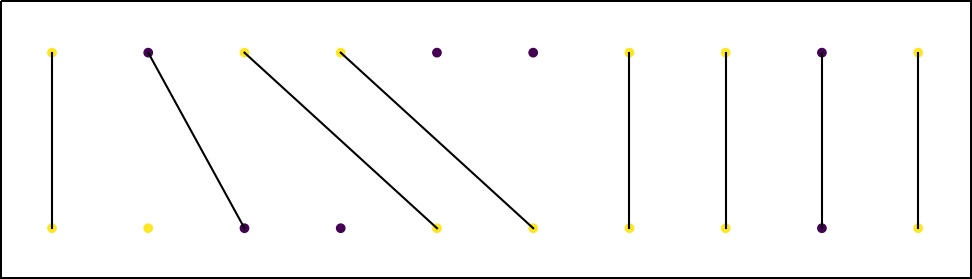
\includegraphics[width=15cm]{lgc} % leia abaixo
\caption{Cada linha horizontal representa uma sequência binária. Dois pontos conectador por uma semi-reta fazem parte de uma maior subsequência.  }
\end{figure}

Note que mudar um elemento de uma das duas subsequências, altera em no máximo $\pm 1$ o valor $Z$, logo, por Efron-Stein \ref{des-efron-stein}:
$$\Var(Z)\leq \dfrac{n}{2}. $$
Logo, por Chebyshev, temos que
$$\pr(|Z-\E(Z)|>\e)\leq \dfrac{n}{2\e^2}, $$
ou seja, a menos de uma constante, $Z$ está a uma taxa de $\sqrt{n}$ do seu valor esperado.




\subsection{Autovalores de Matrizes Aleatórias Simétricas}\index{Autovalores! Matriz Aleatória Simétrica}
Seja $A$ uma matriz simétrica, que tem como entradas v.a.'s $a_{i,j}$, com   $1\leq i\leq j \leq n$ e com valor absoluto limitado por $1$. 

O nosso objetivo é estudar $Z(A)=\lambda_1,$ onde  $\lambda_1$ representa o maior autovalor da matriz aleatória $A$.

\begin{lemma}
Seja $A$ uma matriz simétrica e $\lambda_1$ seu maior autovalor, então
$$\lambda_1 =v^t A v= \sup_{\|x\|=1} x^t A x,$$
onde $v$ é um autovetor associada á $\lambda$, com $\|v\|=1.$
\end{lemma}
\begin{proof}
Como $A$ é simétrica, vamos supor que $A$ é diagonalizável. É claro que se $v$ é um autovalor unitário para $\lambda_1$, então
$$v^t A v = \lambda_1 \|v\|^2 = \lambda_1, $$
e portanto
$$\sup_{\|x\|=1} x^t A x \geq \lambda_1. $$ 
Como $f(x) = x^t A x$ é contínua, então restrita à bola unitária,  ela deve atingir máximo. Suponha que $f$ atinga o máximo em $y$, com $\|y\|=1$. 

Então, se $\lambda_1\geq \dots,\lambda_n$, temos que
\begin{align*}
y^tAy &= \lambda_1y_1^2 + \dots+\lambda_ny_n^2\\
&\leq   \lambda_1y_1^2 + \dots+\lambda_1y_n^2\\
&\leq   \lambda_1(y_1^2 + \dots+y_n^2) = \lambda_1.\\
\end{align*} 
\end{proof}

Agora, vamos utilizar o Teorema \ref{des-efron-stein} da seguinte maneira. Considere $A'_{i,j}$ uma matriz idêntica à $A$, porém substituímos a coordenada $a_{i,j}$ por uma cópia $a'_{i,j}$ independente de $a_{i,j}$. Então, por Efron-Stein, se $v_{i,j}$ é um autovalor unitário para o maior autovalor de $A'_{i,j}$, então
\begin{align*}
(Z-Z'_{i,j})_+ & = ( v^t A v -v_{i,j}^t A'_{i,j} v_{i,j})_+\\
& \leq ( v^tAv -v^tA'_{i,j} v)_+\\
& \leq ( v^t (A-A'_{i,j}) v)_+\\
& = (2 v_iv_j (a_{i,j}-a'_{i,j}))_+\\
& \leq 4 |v_iv_j|. \\
\end{align*}
Portanto,
\begin{align*}
\sum_{1\leq 1\leq j\leq n} (Z-Z'_{i,j})^2_+ &\leq \sum_{1\leq 1\leq j\leq n} 16|v_iv_j|^2\\
&\leq 16\sum_{1\leq 1\leq j\leq n} |v_iv_j|^2\\
&\leq 16\sum_{i=1}^n\sum_{i=1}^n |v_iv_j|^2\\
&\leq 16\left(\sum_{i=1}^n |v_i|^2\right)^2 = 16.\\
\end{align*}
\begin{tcolorbox}[colback = yellow!60]
Ou seja, mostramos que
$$\Var(Z)\leq 16, $$
independente do tamanho da matriz e da distribuição das entradas!
\end{tcolorbox}

\subsection{Valores Singulares de Matrizes Aleatórias}









\newpage
\section{Exercícios Resolvidos}








\chapter{Teoria da Informação}


\begin{tcolorbox}[colback = white]
As Principais referências usadas foram:
\begin{enumerate}
\item \cite{boucheron2013concentration}.
\end{enumerate}
\end{tcolorbox}

\section{Entropia de Shannon e Entropia Relativa}


\begin{definition}[Entropia de Shannon]\index{Entropia! Shannon} Seja $X$ uma v.a. tomando valores num conjunto enumerável com distribuição $p_X$ E entropia de Shannon de $X$ é definida como
$$H(X) = \E(-\ln p_X(X))  = -\sum_{x}p_X(x)\ln p_X(x),$$
com a convenção de que $0\ln 0 = 0.$
\end{definition}

\begin{figure}[h]
\centering % para centralizarmos a figura
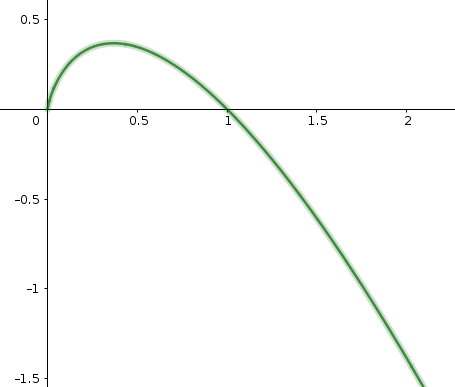
\includegraphics[width=8cm]{xlnx} % leia abaixo
\caption{Gráfico de $x\mapsto -x\ln x.$}
\end{figure}
 



\begin{definition}[Divergência de Kullback-Leibler/ Entropia Relativa]\index{Entropia! Relativa}\index{Divergência de Kullback-Leibler} Sejam $P,Q$ duas probabilidades num conjunto enumerável, com distribuições $p,q$, respectivamente. Então a divergência de Kullback-Leibler ou Entropia Relativa de $P$ e $Q$ é definida como
$$D(P\|Q) = \sum_x p(x)\ln \dfrac{p(x)}{q(x)},$$
se $P$ é absolutamente contínua com respeito à $Q$ e infinito caso contrário. 
\end{definition}


\begin{lemma}
Temos que $D(P\|Q)\geq 0$, valendo a igualdade se, e só se, $P=Q$.
\end{lemma}
\begin{proof}
Lembrando que $\ln x \leq x-1,\ x>0$, temos que
\begin{align*}
D(P\|Q) &= -\sum_x p(x)\ln \dfrac{q(x)}{p(x)}\\
&\geq \sum_x p(x) \left(\dfrac{q(x)}{p(x)}-1 \right)\\
& = \sum_x (q(x)-p(x))\\
& = \sum_x q(x)-\sum_x p(x) = 0.
\end{align*}
E é claro que a igualdade vale se, e só se,  $P=Q$.
\end{proof}

\begin{tcolorbox}[colback = yellow!60]
Vamos analisar o caso específico quando $Q$ é a probabilidade uniforme no espaço base $\Omega$. Temos então que
\begin{align*}
D(P\|Q) &= \sum_x p(x)\ln \dfrac{p(x)}{q(x)}\\
&=\sum_x p(x)\ln\left( |\Omega|p(x)\right)\\
&=\ln|\Omega| - H(X),\\
\end{align*}
onde $X$ é uma v.a. com distribuição $p$.
Do cálculo acima, podemos concluir duas coisas, a primeira é que encontramos uma fórmula explícita para o caso em que $Q$ é uniforme. A segunda é que, como $D(P\|Q)\geq 0$, temos que
$$H(X)\leq \ln|\Omega|, $$
valendo a igualdade se, e só se, $X$ também tem distribuição uniforme sobre $\Omega.$

Isto é, estamos dizendo que a entropia de Shannon é maximizada quando $X$ é uniforme! De certa forma, isso significa que dentre todas as distribuições possíveis, a uniforme é a que menos nos dá 'informação'.
\end{tcolorbox}

\begin{example}
** fazer ex 4.1 e 4.2
\end{example}
\newpage
\section{Entropia em Produtos e Regra da Cadeia}

\begin{proposition}
Sejam $X,Y$ v.a.'s tomando valores num conjunto enumerável. Se $p(x,y)$ é a probabilidade conjunta de $X,Y$ e $p_X,p_Y$ são as probabilidades marginais de $X,Y$, respectivamente, então
$$H(X) + H(Y) - H( (X,Y) ) = \sum_{x,y} p(x,y) \ln \dfrac{p(x,y)}{p_X(x)p_Y(y)}.$$
\end{proposition}
\begin{proof}
Basta lembrar que, por exemplo, para $p_X$, vale
$$p_X(x) = \sum_y p(x,y). $$
\end{proof}

Note que
$$\sum_{x,y} p(x,y) \ln \dfrac{p(x,y)}{p_X(x)p_Y(y)} $$
nada mais é que a entropia relativa da probabilidade conjunta $P$ de $(X,Y)$ e da medida produto $P_X\otimes P_y$, logo 
$$ D(P|P_X\otimes P_y) = H(X) + H(Y) - H( (X,Y) )  \geq 0, $$
valendo a igualdade se, e só se, $X,Y$ são independentes e portanto $P=P_X\otimes P_y$.

\begin{tcolorbox}[colback = yellow!60]
Note que a entropia relativa, ou divergência de Kullback-Leible, funciona como uma distância entre probabilidades. Por exemplo, podemos dizer que  
$$H(X) + H(Y) - H( (X,Y) )\geq 0 $$
mede o quão 'independentes' são $X,Y$.

O valor
$$ H(X) + H(Y) - H( (X,Y) )$$ 
é usualmente conhecido como \emph{informação mutua entre $X$ e $Y$}\index{Informação Mutua}. Note que a entropia de Shannon nada mais é que a informação mutua entre $X$ e $X$. 
\end{tcolorbox}

\begin{definition}[Entropia Condicional] Sejam $X,Y$ duas v.a.'s discretas. Então,
a entropia condicional de $H(X|Y)$  é definida como
$$H(X|Y) = H(X,Y)-H(Y). $$
\end{definition}

Lembrando que $p(x,y) = p(x|y)p_y(y)$, é fácil ver que a definição acima  satisfaz
$$H(X|Y)  = -\E(\ln p(X|Y)),$$
e então, é claro que $H(X|Y)\geq 0.$

Além disso, como 
$$ D(P|P_X\otimes P_y) = H(X) + H(Y) - H( X,Y ), $$
temos que 
$$ D(P|P_X\otimes P_y) = H(X)  - H( X|Y )  \geq 0, $$
ou seja,
$$H(X)\geq H(X|Y), $$
ou seja, a operação de tomar condicional reduz a entropia, o que faz sentido com a nossa intuição de que  condicionar uma v.a. $X$ com respeito à uma $\sigma$-álgebra $\mathcal{F}$, nos dá mais informação sobre $X$.

\begin{proposition}[Regra da Cadeia] Sejam $X_1,\dots,X_n$ v.a.'s, então
\begin{align*}
H(X_1,\dots,X_n) &= H(X_1)+H(X_2|X_1) + H(X_3|X_1,X_2)+\dots\\
&+ H(X_n|X_1,\dots,X_{n-1}). 
\end{align*}
\end{proposition}
\begin{proof}
Façamos o caso em que temos três v.a.'s, o caso geral sai por indução. Através de alguns cálculos simples, conseguimos mostrar que a definição de entropia condicional continua sendo verdade condicionalmente. Temos então que que
$$H(X_3,X_2|X_1) =H(X_2|X_1)+H(X_3|X_1,X_2), $$
somando $H(X_1)$ dos dois lados, temos que
$$H(X_1) + H(X_3,X_2|X_1) = H(X_1)+H(X_2|X_1)+H(X_3|X_1,X_2), $$
mas, utilizando condicionalmente a  definição de entropia condicional,
$$H(X_1) + H(X_3,X_2|X_1) = H(X_1,X_2,X_3). $$
\end{proof}

\begin{tcolorbox}[colback = yellow!60]
Para lembrar da relação $$H(X,Y) = H(X|Y)+H(Y),$$ basta lembrar que
$$P(A,B) = P(A|B)P(B) $$
e que na definição de $H$ há um $\ln$, ou seja, transformamos os produtos em somas.
\end{tcolorbox}
\newpage
\section{Desigualdade de Han}

\begin{theorem}[Desigualdade de Han] \index{Desigualdade! Han} Seja $X_1,\dots,X_n$ uma sequência de v.a.'s discretas. Então
$$H(X_1,\dots,X_n)\leq \dfrac{1}{n-1}\sum_{i=1}^n H(X_1,\dots,X_{i-1},X_{i+1},\dots,X_n). $$
\end{theorem}

\begin{proof}
Note que, dado $0\leq i\leq n$, usando o fato de que $H(X,Y) = H(X|Y)+H(Y)$, temos que
\begin{align*}
H(X_1,\dots,X_n) &= H(X_1,\dots,X_i,\dots,X_n) \\
&= H(X_1,\dots,X_{i-1},X_{i+1},\dots,X_n)+H(X_i|X_1,\dots,X_{i-1},X_{i+1},\dots,X_n).
\end{align*}
Logo, somando em $i$, temos que
\begin{align*}
nH(X_1,\dots,X_n) = \sum_{i=1}^n \left(H(X_1,\dots,X_{i-1},X_{i+1},\dots,X_n)+H(X_i|X_1,\dots,X_{i-1},X_{i+1},\dots,X_n)\right).
\end{align*}
Utilizando o fato de que condicionar reduz a entropia, temos que
$$H(X_i|X_1,\dots,X_{i-1},X_{i+1},\dots,X_n)\leq H(X_i|X_1,\dots,X_{i-1}), $$
mas note que, pela regra da cadeia
$$H(X_1,\dots,X_n) =   \sum_{i=1}^n H(X_i|X_1,\dots,X_{i-1}),$$
e assim concluímos o teorema.
\end{proof}





















\section{Exercícios Resolvidos}






















\bibliographystyle{alpha}

\bibliography{references}\nocite{*}


\newpage

\printindex





\end{document}